\documentclass{practice}

\usepackage{tikz}
\usetikzlibrary{calc,decorations.pathmorphing,shapes,positioning,patterns}

\tcbuselibrary{listings}
\lstset{
basicstyle=\small\ttfamily,
columns=flexible,
breaklines=true
}

\title{2}
\date{\today}

\begin{document}
\maketitle

\begin{task}{Randomness livestream}
  Observe the live flow of your computer's \texttt{/dev/random}.
  Observe then the live flow of \texttt{/dev/urandom}.
  What does your OS's documentation say on the difference between the two?

  Are you running a virtual machine?
  If so, do you think that the quality of VM-internal randomness is affected in any way?
  What does your hypervisor's documentation say about entropy in VMs?
\end{task}

\begin{task}{Testing randomness}
  \textit{Preface.}
  During the lecture we learnt that true randomness is provably unprovable, that is, it has been proven that we cannot prove whether something is truly random.
  While they are not perfect, various test suites exist to statistically evaluate whether some data seems random enough.

  As such, we should keep in mind the following two points:
  \begin{enumerate}
    \item If something does not seem random, that does not prove that it is not random.
    For example, it is possible from time to time for randomness acquired from quality sources to not pass some statistical test.

    In practice, test suites are typically used instead of single tests to evaluate random sequences: the fewer (diverse) tests the data fails, the more likely it is that the data is random.

    \item Randomness test suites are designed to highlight weaknesses in random data, not confirm randomness.
    Passing all tests does not confirm randomness.

    The more elaborate the test suite and the better the testing methodology, the stronger guarantees we have that whatever PRNG was used is not trivially broken.
    Regardless, for cryptographic use (CSPRNG), only generators that have been validated/approved to some degree by cryptographers are suitable.
  \end{enumerate}

  \begin{tcolorbox}[title=Note]
    In cases where we doubt the randomness, or where the randomness seems `weak' for whatever purpose (e.g. you credit card gets the CVC 123), it is often okay to regenerate the values.
    Note, however, that this should not be the norm: the more you reject values based on non-random criteria, the more you introduce bias which could be exploited.
  \end{tcolorbox}

  A quality randomness testing suite is \emph{PractRand}\footnotemark{}.
  \footnotetext{\url{https://pracrand.sourceforge.net}}%
  An alternative is \emph{TestU01}\footnotemark{} but it is harder to set up.
  \footnotetext{\url{https://simul.iro.umontreal.ca/testu01/tu01.html}}%
  \emph{Dieharder}\footnotemark{} is well known and easy to use, but its strength is questionable.
  \footnotetext{\url{https://webhome.phy.duke.edu/~rgb/General/dieharder.php}}

  \textit{Task.}
  Install PractRand and evaluate your computer's current contents of \texttt{/dev/random} with it.
  Note that by default, PractRand will run until the first \enquote{failure} or until it has seen 32TB of data --- manually abort the run after a minute.

  \newtcblisting{commandshell}{listing only,listing options={style=tcblatex,language=sh}}
  %every listing line*={\textcolor{red}{\small\ttfamily\bfseries > }}}

  The commands I used to compile it are:
  \begin{commandshell}
> g++ -std=c++14 -c src/*.cpp src/RNGs/*.cpp \
    src/RNGs/other/*.cpp -O3 -Iinclude -pthread
> ar rcs libPractRand.a *.o
> rm *.o
> g++ -std=c++14 -o RNG_test tools/RNG_test.cpp \
    libPractRand.a -O3 -Iinclude -pthread
  \end{commandshell}

  Then, compile \texttt{rand.c} and evaluate it's output by piping it to PractRand.
  What does the documentation say about C's \texttt{rand()} function?
\end{task}

\begin{task}{Playing the cryptanalyst}
  \textit{Preface.}
  Most programming languages offer some function(s) for generating pseudo-random numbers as part of their standard library.
  Good documentation should always mention whether a method is suitable for producing (pseudo-)randomness of cryptographic quality.
  The rule of thumb is: if the documentation does not mention cryptographic use cases, assume that it is not suitable for cryptographic purposes.

  For Python3, the \texttt{random}\footnotemark{} module can be used to generate \enquote{general purpose} random data, e.g. \texttt{random.randbytes()}.
  \footnotetext{\url{https://docs.python.org/3/library/random.html}}%
  The PRNG uses the \emph{Mersenne-Twister} construction\footnotemark{} (MT), which is a widely used non-cryptographic PRNG due to great statistical properties.
  For example, PractRand will need to parse over 100GB of 32-bit MT data before tests completely fail.
  Still, clever specialised attacks exist against MT making it unsuitable for cryptographic use.%
  \footnotetext{\url{https://en.wikipedia.org/wiki/Mersenne_Twister}}
  
  Most modern programming languages also provide methods for obtaining cryptographically secure pseudo-random numbers.
  Any such functionality must be clearly labelled as such, and even then you should do your research and take the claims with a grain of salt.
  For Python3, cryptographically strong random numbers can be generated with the \texttt{secrets}\footnotemark{} module, e.g. with the \texttt{secrets.token\_bytes()} function.%
  \footnotetext{\url{https://docs.python.org/3/library/secrets.html}}
  Always read the documentation before using functions for cryptography!

  \textit{Recap.}
  Recall the concept of cryptographic distinguishing games, i.e. situations where an adversary must guess which of two scenarios they are in.
  If the adversary has a better success rate than by random guessing---i.e. more than (or less than) $1/2$---we say that the adversary has an \emph{advantage} against the scheme.
  The greater the adversary's advantage, the weaker the scheme.
  An illustration of the flow of the distinguishing game is represented on \autoref{fig:distinguishing}.

  \begin{figure}[h!]
    \centering
    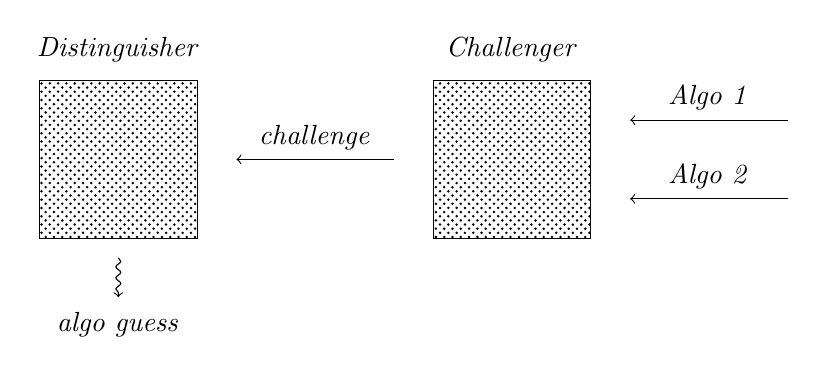
\begin{tikzpicture}[
      Squiggly/.style={
        decorate,
        decoration={snake, segment length=4, amplitude=0.9},
      },
      ]
      \draw[pattern=crosshatch dots] (0, 0) rectangle ++(2,-2);
      \draw[pattern=crosshatch dots] (5, 0) rectangle ++(2,-2);
    
      \node (P) at (1, 0.4) {\textit{Distinguisher}};
      \node (K) at (6, 0.4) {\textit{Challenger}};

      \draw[<-] (7.5, -0.5) -- (9.5, -0.5) node[midway,above] {\textit{Algo 1}};
      \draw[<-] (7.5, -1.5) -- (9.5, -1.5) node[midway,above] {\textit{Algo 2}};
    
      \draw[<-] (2.5, -1) -- (4.5, -1) node[midway,above] {\textit{challenge}};
    
      \draw[->] (1,-2.25) decorate[Squiggly]{ -- (1, -2.75) };
    
      \node (sk) at (1, -3.1) {\textit{algo guess}};
    \end{tikzpicture}
    \caption{The flow of a distinguishing game.}
    \label{fig:distinguishing}
  \end{figure}

  \textit{Task.}
  Your task is to implement the distinguishing game and win it with advantage $\ge 0.8$.
  The following steps outline how to approach this:
  \begin{enumerate}
    \item Implement the challenger:
    \begin{itemize}
      \item Get the challenge size $n$ (in bytes) from the distinguisher.
      \item Randomly sample $n$ bytes of data from either the PRNG (\texttt{random} module) or CSPRNG (\texttt{secrets} module).
      \item Return the data to the challenger.
      \item Return the correct answer (whether it used the PRNG or CSPRNG) to the verifier.
    \end{itemize}
    
    \item Implement the distinguisher:
    \begin{itemize}
      \item Query the challenger for $n$ bytes of challenge,
      \item Process the challenge and try to determine if it comes from the PRNG or CSPRNG.
      
      The file \texttt{mtattack.py} contains the \texttt{recover()} function which, if called correctly, will recover the PRNG from the challenge if it was generated with the Mersenne Twister.
      \item Output the answer to the verifier.
    \end{itemize}

    \item Implement the verifier:
    \begin{itemize}
      \item Ask the distinguisher to run the game many times (e.g. 10).
      \item For each run, get the answer of the distinguisher and of the challenger.
      \item Compute the advantage (the success rate) of the distinguisher.
    \end{itemize}
  \end{enumerate}

  Clearly, if your distinguisher can correctly guess eight out of ten times which of the two generators was used, it has a significant advantage, and you now have empirical proof why you must be careful when choosing your tooling.
\end{task}

\begin{task}{All meanings and no meanings}
  We learnt that the OTP provides information theoretic security, i.e. perfect secrecy, if the key is perfectly random, at least as long as the message, and used only once.

  \textit{Task.}
  Given the OTP ciphertext
  \begin{center}
    \texttt{EE71EBDD2F88923A0115B12E8AB5FC477FFF73894AB25B}
  \end{center}
  and the keys
  \begin{itemize}
    \item \texttt{BA1982AE0FFCF3496A35D85DAAC3993506DF10E625DE7A}
    \item \texttt{AD0392AD5BE7F5486065D957AADC8F671E8816FA25DF3E}
    \item \texttt{B9198AA90FE1E11A757DD40EE9DA8E351A9C07A921D722}
    \item \texttt{BA198EFD5FFAF359757CD24BAADC8F67179E01ED6A8873}
  \end{itemize}
  recovered via brute force, determine which of the keys was the correct key.
  Can you do it with certainty?
  Why yes/why not?
\end{task}

\begin{task}{Two-time pad}
  We learnt that if any of the three properties of the OTP are not respected, the OTP can (and will) fail catastrophically.

  \textit{Task.}
  Below are two OTP ciphertexts (in hex) which were both encrypted with the same key:
  \begin{center}
    \texttt{3C8550F0E566}\hspace*{5em}\texttt{2A925DF2ED74}
  \end{center}
  Both ciphertexts contain a single word of the English dictionary.

  Recover the two words and determine the original message: a concatenation of both words.
  Do you think that your recovered words and/or order are/is correct?
  Can you explain why or why not?

  \textit{Hint.}
  Search for a wordlist online, i.e. a list containing common English words.
  Use this list to help you recover the jumbled words.

  \iffalse
  If you want to check your answers, here is the solution `encrypted' with ROT13 (shift cipher with key 13):
  Gur gjb jbeqf ner lryybj naq benatr, ohg V qb abg rira erzrzore jurgure gur beqre jnf lryybjbenatr be benatrlryybj. Va snpg, vg vf vzcbffvoyr gb erpbire gur beqre bs gur gjb jbeqf (jrer gurl pbapngrangrq va gur pvcuregrkg) fvapr KBE vf pbzzhgngvir, naq obgu pbybhef pbhyq or zrnavatshy. Vg zvtug nyfb or gung gurer rkvfg bgure Ratyvfu jbeqf, be ng yrnfg pbzovangvbaf bs nycunorg yrggref juvpu fngvfsl gur KBE. Fb, juvyr er-hfvat gur xrl oebxr gur cresrpg frperpl, guvf rknzcyr fgvyy cnegyl uvtuyvtugf ubj jryy gur BGC uvqrf vasbezngvba: nyy nafjref juvpu svg ner cbffvoyr.
  \fi
\end{task}

\begin{task}{Beware of the keystream}
  % \textit{Preface.}
  % In the chosen plaintext attack (CPA), an attacker can query the challenger for the encryption of plaintexts of their choice.
  % The more restrictions there are on the attacker's queries (e.g. can only query once), the harder the attack becomes.
  % The challenger acts as, or has access to an encryption oracle, meaning that the challenger can encrypt messages.

  % The attacker's goal is to decrypt the challenge ciphertext, and if possible, optionally recover the key.

  % \textit{Setting.}
  The file \texttt{oracle.py} contains a \enquote{lax} ChaCha20 encryption oracle.
  Lax here denotes that the attacker is allowed to submit the plaintext and the nonce.
  A stricter oracle would randomly select the nonce instead.

  \textit{Task.}
  Given the challenge ciphertext
  \begin{Verbatim}
oIwGebbH+vjzxmy2pDNI94UIkKEZAk2cscdLXnXTDIHCcLbF9A==
  \end{Verbatim}
  encrypted with the nonce \texttt{QPa4aiOwRA0=}, recover the original message (plaintext).
  Note that the secret key is hardcoded into the oracle, but you are not allowed to use it here.

  You need to install the \texttt{pycryptodome}\footnotemark{} package for the oracle to work.
  \footnotetext{\url{https://pypi.org/project/pycryptodome/}}%
\end{task}

\begin{task}{Misuse of a secure cipher}

  [Challenging task]

  \textit{Preface.}
  During the first week I mentioned that it is one thing for a cryptosystem to be secure, but it is another to use it securely in practice.
  Security depends on a lot of conditions, and it should not come as a surprise that using a good key is paramount to the security of a cipher.

  \textit{Setting.}
  Key exchange is complicated, so my friend and I use the following system:
  \begin{enumerate}
    \item We use the UNIX Epoch (without milliseconds) of the message sending time as a seed for our PRNG (\texttt{random.seed()}).
    \item We use the PRNG to generate however many bytes of key material are needed by the cryptosystem (\texttt{random.randbytes()})
    \item We begin every message with `Hey!'.
  \end{enumerate}

  I received the following message from him on the 8\textsuperscript{th} of February 2024 at 13:15:29 GMT+02:00:
  \begin{lstlisting}
  HpHgjwKlYLpxzAdIk8/rYxyVy9/NkNuBJVsk0kOhpuTGq++hjAI90bWeQduo5OOXQY34HF7aOek6GgedJd2npLhhezDO29RF5zzijA==
  \end{lstlisting}

  \textit{Task.}
  Knowing that the message was encrypted with ChaCha20 and the nonce: \texttt{dyYyL8OUw1g=}, what does the message say?

  \textit{Hints.}
  \begin{itemize}
    \item Use the PyCryptodome library.
    \item The ciphertext and seed are base64 encoded.
    \item Read the documentation!
    \item It may have taken a few seconds for me to receive the message.
  \end{itemize}

  P.S. This task is really ridiculous, but if you ever participate in some CTF, this might be the type of nonsense they have you solve.
  Still, there are things to learn from such tasks and hopefully they are also a little fun.
\end{task}

% \begin{tcolorbox}[title=Note]
%   You might have noticed that I use the term \enquote{random numbers} quite loosely.
%   In general, when the context is computers, I of course mean pseudo-random numbers (or bits, bytes, whatever data).
%   I also use the term \enquote{generate}, which makes sense with PRNs, but for TRNs the term \enquote{collect} would likely be more appropriate.
%   Therefore, the rule of thumb is that when I talk about randomness without specifying context, I mean cryptographic quality pseudo-randomness.
% \end{tcolorbox}
\end{document}
